% !TeX encoding = UTF-8
% !TeX spellcheck = es_ES
% !TeX root = ../ComponentCatalog.tex
%!TEX root=../ComponentCatalog.tex

%EC11
\begin{table}[H]
    \centering
    \renewcommand\theadfont{\bfseries}
    \setlength{\tabcolsep}{10pt}
    \renewcommand{\arraystretch}{1.5}

    \begin{tabular}{|c|c|c|c|c|}
        \beginConnectorTable{Encoder EC11}
        \multirow{4}{*}{\makecell{EN11 \\ Suelto}}
        \connectordata{
            \begin{scope}
                \clip (0,0) rectangle  +(2.2,1.5);
                \node[inner sep=0pt] at (0.2,-0.4)
                    {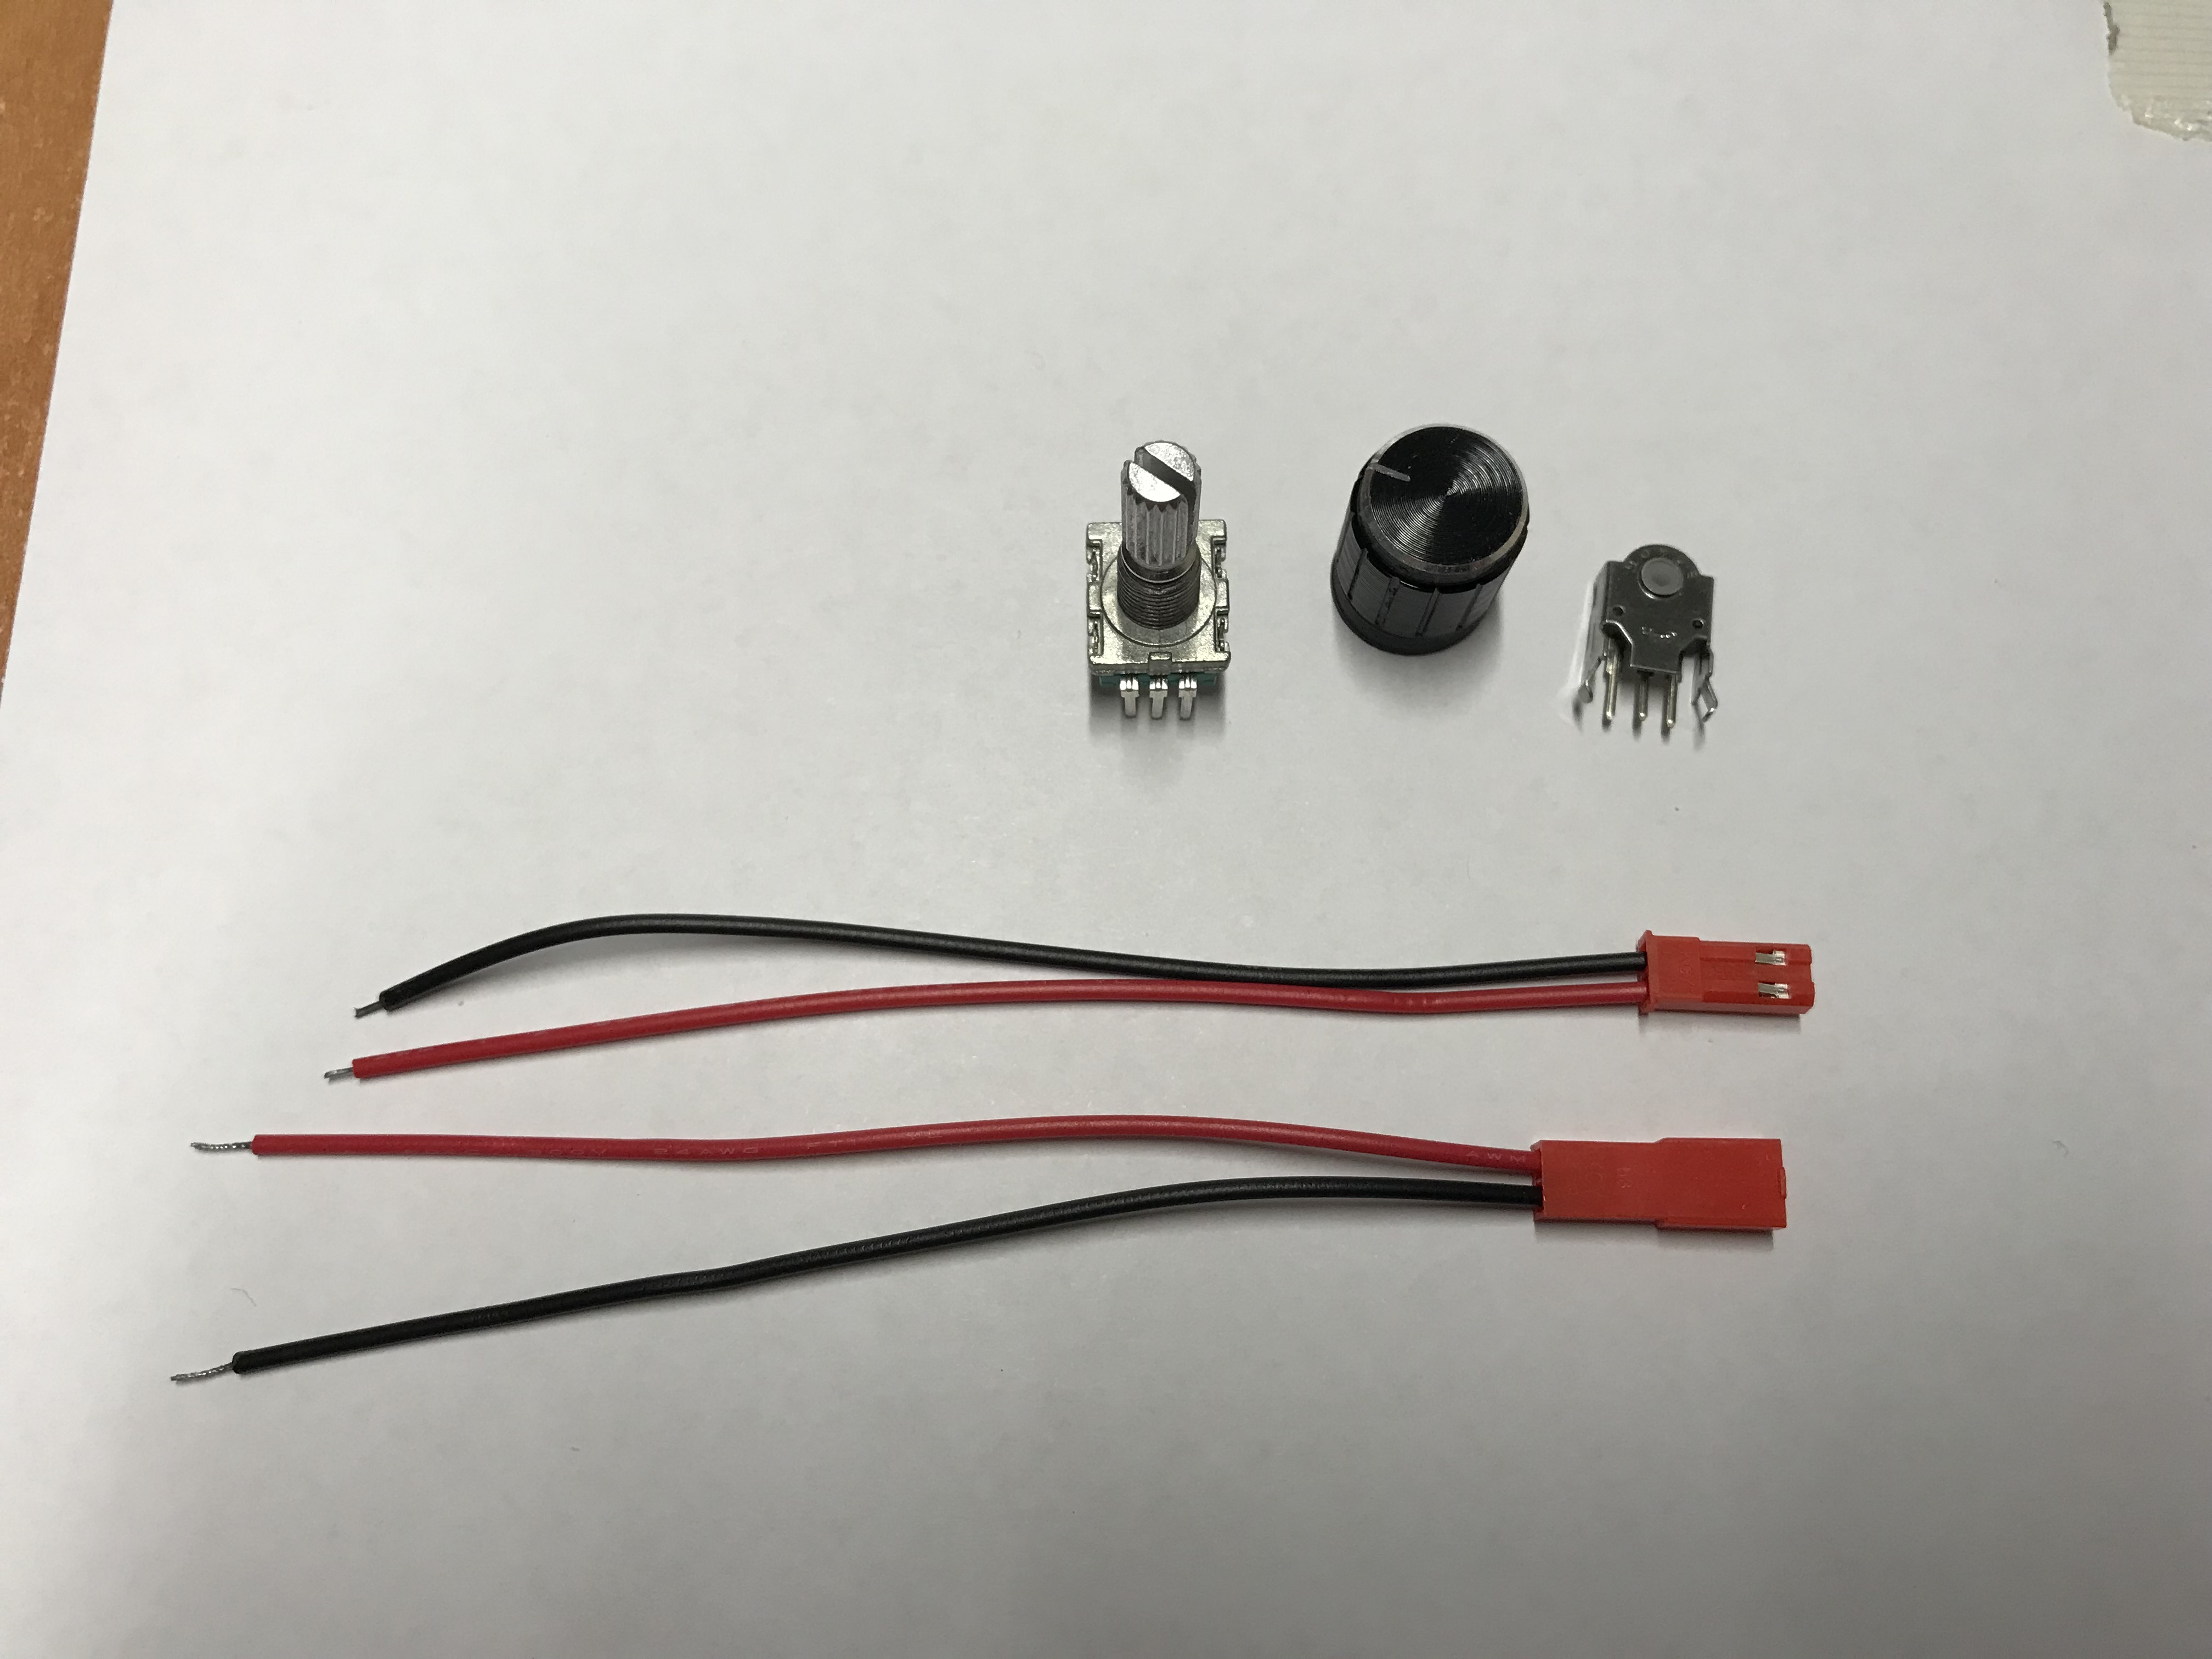
\includegraphics[scale=.07]{pictures/JST.jpg}};
            \end{scope}
        }{
            \draw (0,0) rectangle (3,1.5) ;
        }{Amazon}{EC11} {5V} {10mA} 
        
        \connectorinfo{Codigo}{EN11-HSM1BQ30}{
            \tabitem \textbf{Fabricante}: TT Electronics
        }
        \cline{1 - 2}
        \connectorblockinfo{Uso}{UI Dcc Decoder Config}
        \connectorblockinfo{Ubicacion}{Terraza}
    \end{tabular}
    \caption{Encoder EC11}
    \label{tab:EC11}
\end{table}

%Mouse
\begin{table}[H]
    \centering
    \renewcommand\theadfont{\bfseries}
    \setlength{\tabcolsep}{10pt}
    \renewcommand{\arraystretch}{1.5}

    \begin{tabular}{|c|c|c|c|c|}
        \beginConnectorTable{Encoder Raton}
        \multirow{3}{*}{\makecell{EC10 }}
        \connectordata{
            \begin{scope}
                \clip (0,0) rectangle  +(1.3,1.4);
                \node[inner sep=0pt] at (-2.8,-0.5)
                    {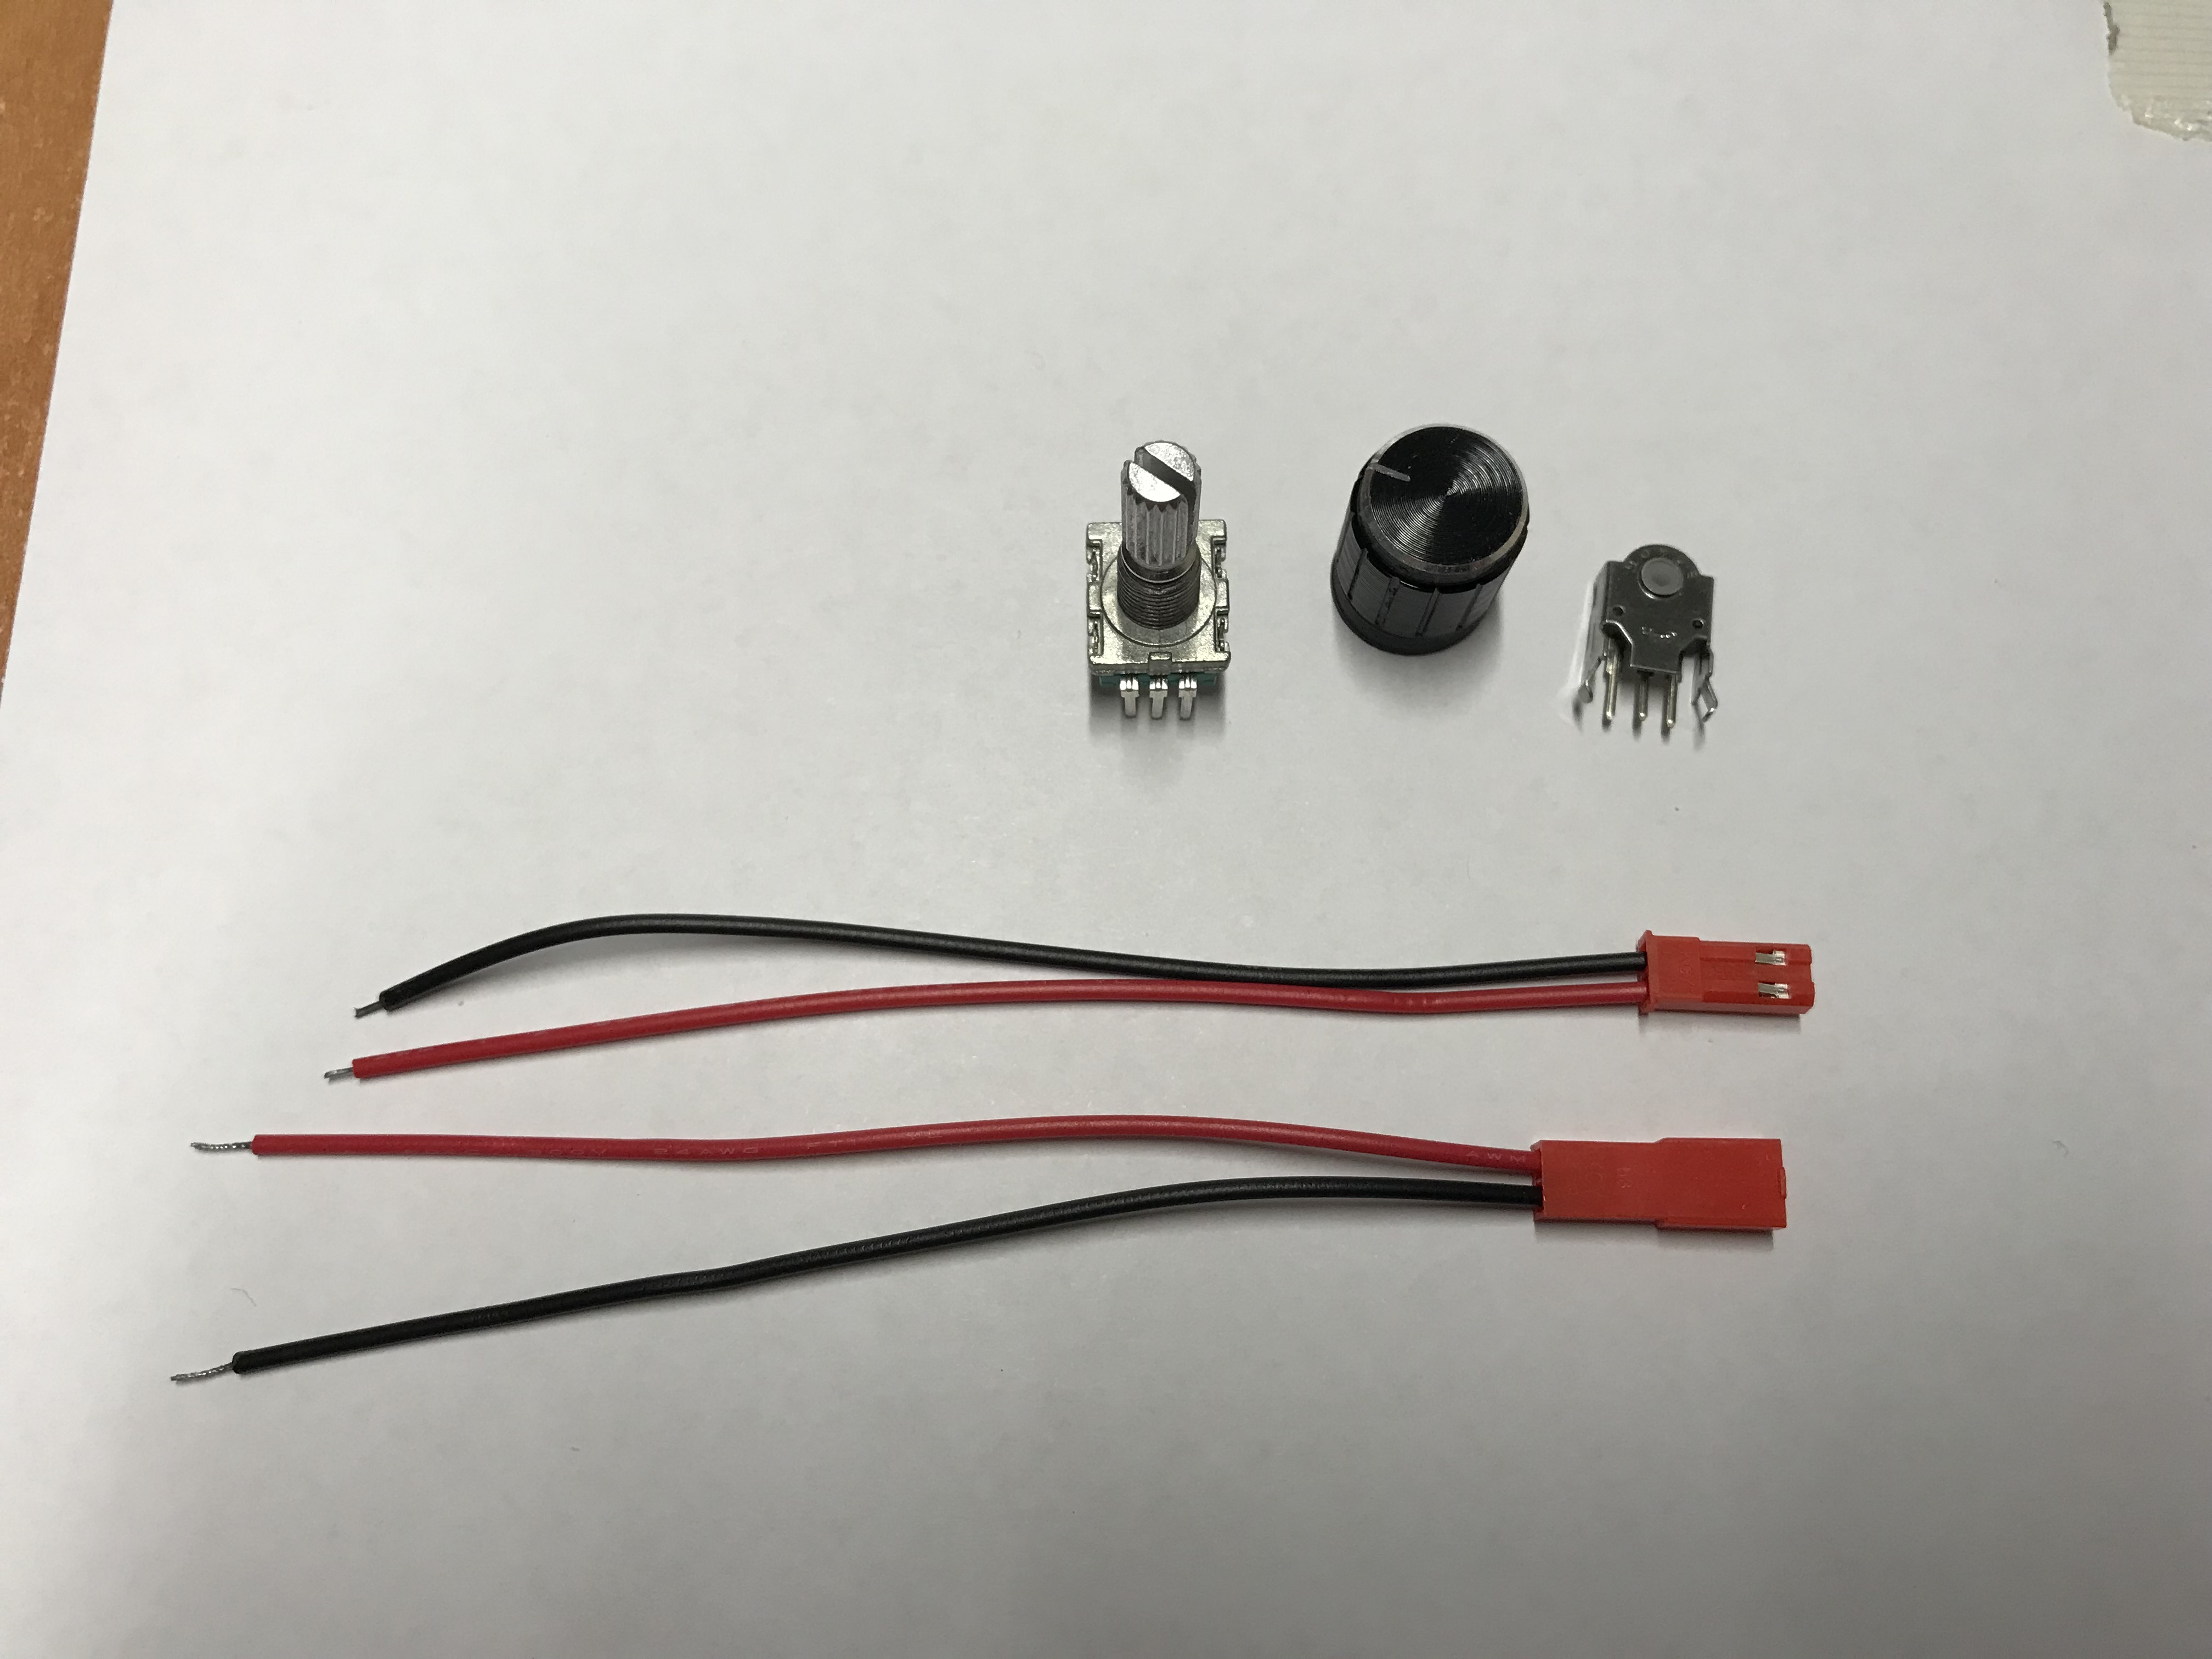
\includegraphics[scale=.1]{pictures/JST.jpg}};
            \end{scope}
        }{
            \draw (0,0) rectangle (3,1.5) ;
        }{Aliexpress}{Codificador} {5V} {1mA} 
        
        \connectorinfo{Codigo}{EN11-HSM1BQ30}{
            \tabitem \textbf{Fabricante}: ALPS
        }
        \cline{1 - 2}
        \connectorblockinfo{Uso}{UI Dcc Decoder Config}
        \connectorblockinfo{Ubicacion}{Terraza}
    \end{tabular}
    \caption{Encoder EC10}
    \label{tab:EC10}
\end{table}